\section{Case Study}
\label{sec:cs}

To demonstrate how \sysname{} works and to detail how a complex distributed
application can be specified in \sysname{} for the compatibility check with
pluggable distributed services, we conduct case studies of three applications.
Two applications, a movie streaming service and an online shopping
mall, are from
a microservice benchmark suite~\cite{gan2019an} and the other is from an
academic system that designs causally consistent storage service
across multiple weakly consistent distributed storage services~\cite{boltoncc}.
We mainly focus on the movie example to delve into the details.
Our framework is designed for a quick specification of applications
and prompt compatibility checks, and assumes users to be familiar with
axiomatic semantics and SMT encodings.

\subsection{Movie Streaming Service}

Our movie streaming service application~\cite{gan2019an} involves
multiple functionalities that can be represented as
regular nodes and edges in \sysgraph{} and distributed storage services (or DBs)
that can be captured as \sysmods{} (\cref{fig:case-study-media}).

\para{System Architecture}
The media streaming service consists of eleven interconnected
components, each with specific consistency requirements based on
their functional roles. While users can choose a \sysmod{} for the
DB components, they must specify the constraints for the other components.

\begin{figure}[h]
  \centering
  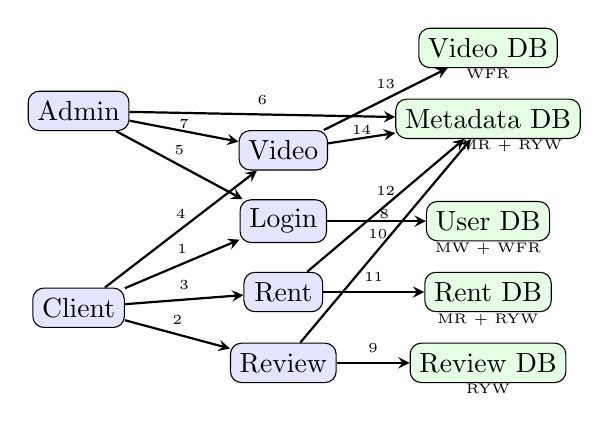
\begin{tikzpicture}[
      node distance=1.8cm,
      service/.style={draw, rounded corners, fill=blue!10, minimum
      width=1cm, minimum height=0.5cm},
      storage/.style={draw, rounded corners, fill=green!10, minimum
      width=1cm, minimum height=0.5cm},
      arrow/.style={->, >=stealth, thick},
      label/.style={font=\small\itshape}
    ]
    % client and admin
    \node[service] (client) at (0,0) {Client};
    \node[service, yshift=3mm] (admin) at (0,2.2) {Admin};

    % services
    \node[service] (login) at (2.6,1.1) {Login};
    \node[service] (review) at (2.6,-0.7) {Review};
    \node[service] (rent) at (2.6,0.2) {Rent};
    \node[service] (video) at (2.6,2.0) {Video};

    % db nodes
    \node[storage] (user_db) at (5.2,1.1) {User DB};
    \node[storage] (metadata_db) at (5.2,2.4) {Metadata DB};
    \node[storage] (review_db) at (5.2,-0.7) {Review DB};
    \node[storage] (rent_db) at (5.2,0.2) {Rent DB};
    \node[storage] (video_db) at (5.2,3.3) {Video DB};

    % edges from client with centered, above labels
    \draw[arrow] (client) -- (login) node[pos=0.5, above, font=\tiny] {1};
    \draw[arrow] (client) -- (review) node[pos=0.5, above, font=\tiny] {2};
    \draw[arrow] (client) -- (rent) node[pos=0.5, above, font=\tiny] {3};
    \draw[arrow] (client) -- (video) node[pos=0.5, above, font=\tiny] {4};

    % edges from admin
    \draw[arrow] (admin) -- (login) node[pos=0.5, above, font=\tiny] {5};
    \draw[arrow] (admin) -- (metadata_db) node[pos=0.5, above, font=\tiny] {6};
    \draw[arrow] (admin) -- (video) node[pos=0.5, above, yshift=-1mm,
    font=\tiny] {7};

    % service to DB edges
    \draw[arrow] (login) -- (user_db) node[pos=0.5, above,
    xshift=1mm, yshift=-1mm, font=\tiny] {8};
    \draw[arrow] (review) -- (review_db) node[pos=0.5, above, font=\tiny] {9};
    \draw[arrow] (review) -- (metadata_db) node[pos=0.5, above,
    xshift=-1mm, yshift=-1mm, font=\tiny] {10};
    \draw[arrow] (rent) -- (rent_db) node[pos=0.5, above, font=\tiny] {11};
    \draw[arrow] (rent) -- (metadata_db) node[pos=0.5, above, font=\tiny] {12};
    \draw[arrow] (video) -- (video_db) node[pos=0.5, above, font=\tiny] {13};
    \draw[arrow] (video) -- (metadata_db) node[pos=0.5, above,
    yshift=-0.8mm, font=\tiny] {14};

    % semantics for databases only
    \node[below=0.15cm, align=center, font=\tiny] at (user_db) {MW + WFR};
    \node[below=0.15cm, align=center, xshift=3mm, font=\tiny] at
    (metadata_db) {MR + RYW};
    \node[below=0.15cm, align=center, font=\tiny] at (review_db) {RYW};
    \node[below=0.15cm, align=center, font=\tiny] at (rent_db) {MR + RYW};
    \node[below=0.15cm, align=center, font=\tiny] at (video_db) {WFR};
  \end{tikzpicture}
  \caption{Architecture of the media streaming service with
    consistency guarantees.
    Edges are numbered for reference:
    1–4: Client requests to services (login, review, rent, video).
    5: Admin login.
    6: Admin updates metadata.
    7: Admin uploads video.
    8: Login service accesses User DB.
    9: Review service writes to Review DB.
    10: Review checks content existence in Metadata DB.
    11: Rent updates Rent DB.
    12: Rent checks content availability in Metadata DB.
    13: Video service accesses Video DB.
  14: Video service verifies metadata before playback.}
  \label{fig:case-study-media}
\end{figure}

\begin{enumerate}[leftmargin=*,noitemsep,topsep=2pt]
  \item \textbf{Client and Admin}: These components represent the
    entry points for regular users and administrative personnel,
    respectively. They don't enforce specific consistency guarantees
    themselves but rely on the guarantees provided by the services
    they interact with.

  \item \textbf{Authentication}:
    \begin{itemize}[leftmargin=*, noitemsep,topsep=0pt]
      \item \textbf{Login Service}: Manages user authentication and
        session handling. It requires order preserving writes
        for correct credential update and the user's updates
        (e.g., subscription status change) must always be visible for
        flawless service.
      \item \textbf{User DB}: Stores user credentials and
        profile information.
        %MW and WFR ensures
        %that when users update their profiles or credentials, these
        %changes are consistently visible to subsequent operations.
    \end{itemize}

  \item \textbf{Content Management}:
    \begin{itemize}[leftmargin=*, noitemsep,topsep=0pt]
      \item \textbf{Video Service}: Handles video streaming requests
        and requires users to see what they already saw to ensure
        consistent content delivery.
      \item \textbf{Metadata DB}: Stores information about
        available media content (titles, descriptions, genres, etc.).
        %        with Monotonic Reads (MR) and Read Your Writes (RYW)
        %        guarantees. This allows administrative updates to be
        %        immediately visible while tolerating some staleness
        % for user reads.
      \item \textbf{Video DB}: Stores the actual video content
        with WFR guarantees to maintain version consistency.
    \end{itemize}

  \item \textbf{User-Centered Functions}:
    \begin{itemize}[leftmargin=*, noitemsep,topsep=0pt]
      \item \textbf{Review Service}: Manages user reviews and
        requires users to immediately see their own reviews.
      \item \textbf{Review DB}: Stores user reviews.
        %with RYW
        %guarantees, allowing users to see their own reviews
        %immediately while other users might see slightly stale data.
      \item \textbf{Rent Service}: Handles media rental transactions
        and requires users to see their activities immediately.
      \item \textbf{Rent DB}: Records rental transactions.
        %with MR and RYW guarantees to maintain consistent transaction history.
    \end{itemize}
\end{enumerate}

\para{Constraint Encoding.}
In this example, the application requires that all users must register for
an account before they can log in, this would result in a request from
client to login service (edge 1), then to user database (edge 8).
If users want to post a review (edge 2), they must
be logged in (edge 1), and the review service must verify that the
title exists
in the metadata database (edge 10) before allowing the review to be
written (edge 9).
This is one of the clear dependency chains in the media service example.
This dependency chain creates a cascading effect throughout the system
where each operation builds upon the successful completion of its
prerequisites.
The registration-before-login dependency establishes user identity,
the login-before-content-access dependency establishes authorization,
and the content-validation-before-review dependency establishes
referential integrity.

Semantically, 6 nodes are interacting with each other (client,
  login service, user database, review service, metadata database,
and review database) in the aforementioned dependency chain.
The edges between these nodes represent the flow of API requests and we
encode the prerequisites of each request as constraints on edges.
Implementation-wise, all constraints on edges can be
directly encoded on the nodes themselves along with our
predefined semantics. However, when modeling
services with complex interactions with cross storage system
dependencies, edge constraints can clearly
separate the providing/requiring semantic constraints from downstream
implementation-specific
service logic. In the implementation, we defined multiple operations
with read or write type to represent interactions between client,
service nodes, and storage nodes.
Formally, we can represent client's login operation (edge 8) as follows:

% old version with linefeed
% \begin{align*}
%   EC_{login} &\triangleq \forall op_{login} \in H_{rd} : \exists
%   op_{reg} \in H_{wr} :\\
% &ob(op_{login}, op_{reg}) \land vis(op_{reg}, op_{login}))
% \end{align*}
% new version wo linefeed and consistent notation
\[
  EC_{\text{login}} \triangleq \forall op_{\text{login}} \in H_{\text{rd}} : \exists op_{\text{reg}} \in H_{\text{wr}} :
  (op_{\text{login}}, op_{\text{reg}}) \in ob \land (op_{\text{reg}}, op_{\text{login}}) \in vis
\]

Since all interactions to User DB pass through Login, and Login node do not have cross
edges to outside graph components other than User DB, the subgraph Login, User DB and
edge 8 can be aggregated with \texttt{extract} function.

For services initiated from the client side, we modeled the behaviors
as a set of re-useable common constraints with the return-before
binary relationship. Formally:

% old version with linefeed
% \begin{align*}
% EC_{auth} &\triangleq rb(op_{login}, op_{rdreview}) \land
% rb(op_{login}, op_{wrreview}) \\
% &\land rb(op_{login}, op_{rent}) \land rb(op_{login}, op_{watch})
% \end{align*}
% new version with linefeed and consistent notation
% this is too wide
\begin{align*}
  EC_{\text{auth}} &\triangleq
  (op_{\text{login}}, op_{\text{rdreview}}) \in rb \land
  (op_{\text{login}}, op_{\text{wrreview}}) \in rb \\ &\land
  (op_{\text{login}}, op_{\text{rent}}) \in rb \land
  (op_{\text{login}}, op_{\text{watch}}) \in rb
\end{align*}

The common constraints are then added to each edge that is dependent on the
login service or refer to the login operation, ensuring the chain
of dependencies is respected throughout the system.

For posting reviews,
the review service must first verify that the content exists in the
metadata database before allowing the review to be written. Similar to
the login operation, we can represent the review service's interaction
as a set of constraints with existential quantification, object constraints,
and return-before relationships, on top of consistency semantics
encoded at each nodes' provide and need fields.

\begin{align*}
EC_{\text{review}} &\triangleq \forall op_{\text{review}} \in H_{\text{wr}} : \exists op_{\text{rdmeta}} \in H_{\text{rd}} :\\
&(op_{\text{review}}, op_{\text{rdmeta}}) \in ob \land (op_{\text{rdmeta}}, op_{\text{review}}) \in rb
\end{align*}

Following these practices one can specify relatively complex and construct \sysgraph with \sysmods and application-level constraints.

%The example already specifies satisfiable \sysmods{}, but users can
%test other \sysmods{} or ask \sysname{} to search for the compatible
% \sysmods{}.

\para{Requirements and Compatibility Verification.}
Each component in the system requires consistency guarantees
from the DBs:% based on its functional role:
\begin{itemize}
\item The User DB provides MW and WFR guarantees, ensuring
  that credential updates are properly sequenced and visible, which
  is critical for authentication security.
\item The Metadata DB provides MR and RYW guarantees,
  balancing immediate visibility of administrative updates with
  tolerance for some staleness in user reads.
\item The Review DB provides RYW guarantees, prioritizing the
  user experience of seeing one's own reviews immediately while
  accepting eventual consistency for other users' views.
\item The Rent DB provides MR and RYW guarantees, ensuring
  consistent transaction records for both administrative and user views.
\item The Video DB provides WFR guarantees, maintaining
  version consistency for content delivery.
\end{itemize}

The edges in our model represent not just data flow but also critical
operational constraints. For example, the edge from the Client to the
Login Service carries the constraint that "User must register before
login," enforced through a visibility relationship between
registration and login operations. Similarly, the edge from the
Review Service to the Metadata Database enforces the constraint that
"Check metadata before reading reviews," ensuring that reviews are only
accessible for valid content.

When we apply the \texttt{composable} function to this system,
starting from the client node, it successfully verifies that the
composition of these services with their respective consistency
guarantees satisfies the overall system requirements.
This verification confirms that despite the heterogeneous consistency
guarantees across different components, the system as a whole
maintains its required properties.
%For instance, the login flow
%correctly enforces that registration must precede login, and the
%review system correctly ensures that users can immediately see their
%own reviews while maintaining content validity checks.

\subsection{Online Shopping Mall}

An e-commerce application~\cite{gan2019an} is similar to the movie
streaming service but its architecture and constraints are simpler
(\cref{fig:case-study-shop}).

\para{Architecture.}
The online shopping application consists of five key components and only
models client behaviors:

\begin{figure}[t]
\centering
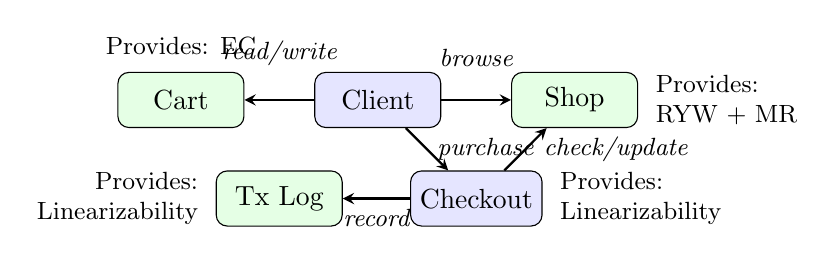
\begin{tikzpicture}[
    node distance=1.2cm,
    service/.style={draw, rounded corners, fill=blue!10, minimum
    width=1.6cm, minimum height=0.7cm},
    storage/.style={draw, rounded corners, fill=green!10, minimum
    width=1.6cm, minimum height=0.7cm},
    arrow/.style={->, >=stealth, thick},
    label/.style={font=\small\itshape}
  ]

  % nodes
  \node[service] (client) at (-0.3,0) {Client};
  \node[storage] (cart) at ([shift={(180:2.5cm)}]client) {Cart};
  \node[storage] (shop) at ([shift={(0:2.5cm)}]client) {Shop};
  \node[service] (arbitrator) at ([shift={(315:1.77cm)}]client)
  {Checkout};
  \node[storage] (tx) at ([shift={(225:1.77cm)}]client) {Tx Log};

  % edges
  \draw[arrow] (client) -- (cart) node[midway, above=0.3cm,
  label] {read/write};
  \draw[arrow] (client) -- (shop) node[midway, above=0.3cm, label] {browse};
  \draw[arrow] (client) -- (arbitrator) node[midway, right, label]
  {purchase};
  \draw[arrow] (arbitrator) -- (shop) node[pos=0.3175,
  right=0.2cm, yshift=0.1cm, label] {check/update};
  \draw[arrow] (arbitrator) -- (tx) node[midway, below, label] {record};

  % semantics
  \node[above=0.1cm, align=center, font=\small] at (cart.north)
  {Provides: EC};
  \node[right=0.1cm, align=left, font=\small] at (shop.east)
  {Provides:\\RYW + MR};
  \node[right=0.1cm, align=left, font=\small] at (arbitrator.east)
  {Provides:\\Linearizability};
  \node[left=0.1cm, align=right, font=\small] at (tx.west)
  {Provides:\\Linearizability};
\end{tikzpicture}
\caption{Architecture of the online shopping system with
consistency guarantees}
\label{fig:case-study-shop}
\end{figure}

\begin{enumerate}[leftmargin=*, noitemsep,topsep=0pt]
\item \textbf{Client}: The end-user interface through which
  customers browse products, manage their shopping cart, and
  initiate purchases. The client itself doesn't enforce specific
  consistency guarantees but relies on the guarantees provided by
  the services it interacts with.

\item \textbf{Cart DB}: The shopping cart DB maintains customers'
  shopping cart state. It stores items that customers intend to
  purchase and supports read and write operations. The cart can be
  loosely managed and immediate propagation of updates is not required.

\item \textbf{Shop DB}: Maintains the authoritative inventory state
  for all products. Clients can observe stale state, but the shop must provide
  up-to-date information to the checkout service which process purchase
  transactions.

\item \textbf{Checkout}: Acts as a serialization point for
  purchase transactions, providing linearizability guarantees. This
  critical component ensures that concurrent purchase requests are
  processed in a well-defined sequence, preventing race conditions
  that could lead to inventory inconsistencies or duplicate transactions.
  Even if it works with DBs that guarantee weaker semantics than
  linearizability,
  its logic should guarantee strong consistency.

\item \textbf{Tx Log DB}: Records all completed purchases
  with linearizability guarantees, ensuring that transaction
  records are stored in a strictly consistent manner for auditing
  and financial reconciliation purposes.
\end{enumerate}

%\subsubsection{Interaction Flow}
%
%The typical interaction flow in this system follows several patterns:
%
%\textbf{Browsing and Cart Management:} Customers interact directly
%with the shop service to browse available products. When they find
%items of interest, they can add these items to their cart through the
%cart service. These operations don't require strong consistency
%guarantees as they don't modify the authoritative inventory state.
%
%\textbf{Purchase Process:} When a customer decides to complete their
%purchase, a more complex interaction begins:
%
%\begin{enumerate}
%  \item The client sends a purchase request to the arbitrator,
%    including the contents of the customer's cart.
%
%  \item The arbitrator, acting as a serialization point, first reads
%    from the shop's inventory to verify that all requested items are
%    available in sufficient quantities.
%
%  \item If the inventory check succeeds, the arbitrator performs two
%    operations in sequence:
%    \begin{itemize}
%      \item It writes to the shop service to decrement the inventory
%        counts for the purchased items.
%      \item It writes to the transaction log to record the successful
%        purchase, capturing details such as items purchased,
%        quantities, prices, and customer information.
%    \end{itemize}
%
%  \item If the inventory check fails (e.g., an item is out of stock),
%    the arbitrator responds to the client with an error message, and
%    no changes are made to either the inventory or transaction log.
%\end{enumerate}
%
%This interaction pattern ensures that inventory updates and
%transaction records are kept in sync, preventing scenarios where
%inventory is decremented without a corresponding transaction record
%or vice versa.

\para{Requirements and Compatibility Verification}
The consistency requirements of this system vary by component:

\begin{itemize}
\item The shop DB provides RYW and MR, which are sufficient for
  a centralized Checkout service to manage inventory.
  RYW ensures that once the Checkout updates inventory levels,
  any subsequent reads will observe these updates. MR ensures that
  if a client observes a certain inventory state, all subsequent
  reads will observe either that same state or a more recent one,
  but seeing outdated state is okay as Checkout will prevent
  ill-formed purchase transaction (e.g., purchasing out-of-stock item).

\item Checkout and transaction log DB both provide
  linearizability, the strongest consistency model, ensuring that
  all operations appear to execute atomically in a sequential order
  that is consistent with the real-time ordering of those
  operations. This is critical for the financial aspects of the system.

\item The cart service has more relaxed consistency requirements,
  as temporary inconsistencies in cart state don't impact the
  integrity of the inventory or financial records.
\end{itemize}

An interesting aspect of this example is that Checkout can guarantee
linearizability as long as it is the sole entry updating the Shop DB.
The verification confirms that Checkout's linearizability
guarantee is sufficient to coordinate between the shop's RYW+MR
guarantees and the transaction log's linearizability, ensuring that
inventory updates and transaction records remain consistent even
under concurrent operations.

\begin{figure}[t]
\centering
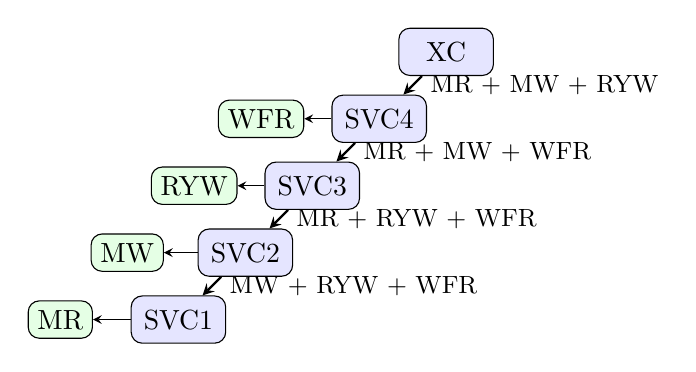
\begin{tikzpicture}[
    node distance=1.2cm,
    service/.style={draw, rounded corners, fill=blue!10, minimum
    width=1.2cm, minimum height=0.6cm},
    semantic/.style={draw, rounded corners, fill=green!10, minimum
    width=0.8cm, minimum height=0.4cm},
    arrow/.style={->, >=stealth, thick},
    semantic_arrow/.style={->, >=stealth, thin},
    label/.style={font=\small}
  ]

  % nodes positioned at 45 degree angle upward
  \node[service] (svc1) at (0,0) {SVC1};
  \node[service] (svc2) at (0.85,0.85) {SVC2};
  \node[service] (svc3) at (1.7,1.7) {SVC3};
  \node[service] (svc4) at (2.55,2.55) {SVC4};
  \node[service] (xc) at (3.4,3.4) {XC};

  % semantic nodes at same level as their corresponding services
  \node[semantic] (mr) at (-1.5,0) {MR};
  \node[semantic] (mw) at (-0.65,0.85) {MW};
  \node[semantic] (ryw) at (0.2,1.7) {RYW};
  \node[semantic] (wfr) at (1.05,2.55) {WFR};

  % arrows from services to semantics
  \draw[semantic_arrow] (svc1) -- (mr);
  \draw[semantic_arrow] (svc2) -- (mw);
  \draw[semantic_arrow] (svc3) -- (ryw);
  \draw[semantic_arrow] (svc4) -- (wfr);

  % edges
  \draw[arrow] (svc2) -- (svc1);
  \draw[arrow] (svc3) -- (svc2);
  \draw[arrow] (svc4) -- (svc3);
  \draw[arrow] (xc) -- (svc4);

  % edge constraints (horizontal text, right of edges)
  \node[right=0.1cm, font=\small] at (0.425,0.425) {MW + RYW + WFR};
  \node[right=0.1cm, font=\small] at (1.275,1.275) {MR + RYW + WFR};
  \node[right=0.1cm, font=\small] at (2.125,2.125) {MR + MW + WFR};
  \node[right=0.1cm, font=\small] at (2.975,2.975) {MR + MW + RYW};

\end{tikzpicture}
\caption{Cross-service causal consistency composition chain}
\label{fig:cross-service-causal}
\end{figure}

\subsection{Cross Causal (XC) Storage}
Cross causal (XC) storage~\cite{boltoncc} is a system that combines
multiple distributed storage services, each
offering only a basic consistency guarantee, to provide causal consistency
as a whole (\cref{fig:cross-service-causal}).
Users accessing data through the XC node can expect to get causal consistency,
but individual storage DB maintains weaker semantics than causal.
SVC4 node's storage backend only provides WFR. To achieve causal
consistency, application places a shim layer to strengthen the semantics
in the design and this is imposed on the edge between SVC4 and XC.
While the SVC4-XC combination can achieve causal consistency, SVC4's
downstream service
node SVC3's storage backend only provides RYW. Again, to achieve
cross-system causal consistency, the augmentation continues down the chain.

%This example demonstrates modeling a system where multiple services, each
%offering only a basic consistency guarantee, are chained together.

The goal here is to verify if their composition, mediated by specific
inter-service
constraints, symbolic isolation, and the role of explicit ``glue'' constraints.

\para{Architecture.} The architecture forms a chain $\text{XC} \rightarrow
\text{SVC4} \rightarrow \text{SVC3} \rightarrow \text{SVC2}
\rightarrow \text{SVC1}$.
Each service $\text{SVC}n$ (for $n=1..4$) is designed to provide only
\textit{one} of the
four session guarantees via its \texttt{provs} attribute:
$\text{SVC}1$ provides MR, $\text{SVC}2$ provides
MW, $\text{SVC}3$ provides RYW, and $\text{SVC}4$ provides WFR.

\para{Constraints Encoding and Compatibility Verification.}
%\textbf{Symbolic Isolation:}
To prevent logical interference, the guarantee provided by
each service and the constraints added on the edges are instantiated
using unique
symbols specific to that service or edge.
This ensures, for example, that the MR constraints of
$\text{SVC}1$ only apply to operations symbolically designated as belonging to
$\text{SVC}1$.

%\textit{Composition via Edge Constraints:}
The composition logic resides in the ``glue''
constraints defined on the \texttt{cons} attribute of the edges connecting the
services. Since each service node only provides one session
guarantee, the edge $\text{SVC}n \rightarrow \text{SVC}(n+1)$ must
provide constraints representing the other three session guarantees needed to
potentially satisfy causal consistency up to that point.

The core idea of this example is to build a stronger guarantee by composing
weaker guarantees provided by individual services ($\text{SVC}1
\ldots 4$), using
the edges to supply the missing pieces which reflects the application design
as shown in \cref{fig:cross-service-causal}.

%\begin{itemize}
%\item $\text{SVC}1$ provides only MR via its storage backend.
%\item To achieve Causal Consistency when accessing data through $\text{SVC}2$,
%  the edge between $\text{SVC}1$ and $\text{SVC}2$ must
%  provide the missing session guarantees: MW, RYW, and WFR through
%  application-level business logic.
%\item Similarly, $\text{SVC}2$ provides only MW via its storage
%  backend. To maintain Causal Consistency
%  when accessing data through $\text{SVC}3$, the edge between
%  $\text{SVC}2$ and $\text{SVC}3$ must
%  provide MR, RYW, and WFR.
%\item This pattern continues: $\text{SVC}3$ provides RYW, so the edge
%  to $\text{SVC}4$ must provide MR, MW, and WFR.
%\item Finally, $\text{SVC}4$ provides WFR, so the edge to $\text{XC}$
%  must provide MR, MW, and RYW.
%\item The $\text{XC}$ node serves as the extraction point where users
%  can access data with full causal consistency guarantees.
%\end{itemize}

%\textit{Symbol Equivalence:}
For this composition to be meaningful in the SMT-solver-based
\sysname{}, we must
conceptually link operations across services that refer to the same logical
action or data. For instance, if write $w_1$ in $\text{SVC}1$ and
write $w_2$ in $\text{SVC}2$ both
represent updates to the same user profile, ``glue'' constraints
equating relevant
aspects (like $w_1.\text{obj} = w_2.\text{obj}$ or $w_1.\text{ival} =
w_2.\text{ival}$ despite their different symbolic names) is necessary.
While the current test code
simplifies this by focusing on composing the consistency axioms, a more rigorous
model would include these explicit symbol equivalence constraints on the edges
(we are directly asserting symbols of $w_1$ are identical to those of $w_2$ for
simplicity).

%\textit{Aggregation:} The \texttt{composable(g, svc1)} call attempts
%to find a satisfying
%assignment for the entire chain, respecting the \texttt{provs} of
%each node and the \texttt{cons} of
%each edge. If it returns \texttt{True}, it confirms that the
%individual guarantees can
%be composed under the specified edge constraints. Subsequently,
%\texttt{extract(svc1, svc1, (ok, res))} can

After a single logical formula representing the net end-to-end guarantee
achieved by the SVC chain is synthesized starting from $\text{SVC}1$
to XC, the formula is then compared against a formal definition of CC
to verify compatibility, which succeeds. While
the original XC implementation~\cite{boltoncc} ties together only EC
storage services, this example further explores more diverse storage
services and demonstrates the flexibility of \sysname{}.
%\subsubsection{Interaction Flows}
%
%The media streaming service supports several interaction patterns,
%each with specific consistency requirements:
%
%\textbf{User Registration and Authentication}: Before accessing any
%content, users must register and authenticate through the login
%service. This process involves:
%
%\begin{enumerate}
%\item The client sends a registration request (abstracted as a
%  write operation) to the login service.
%\item The login service writes the new user credentials to the User Database.
%\item For subsequent logins, the client sends a login request
%  (abstracted as a read operation) to the login service.
%\item The login service reads from the User Database to verify credentials.
%\end{enumerate}
%
%The MW and WFR guarantees of the User Database ensure that once user
%credentials are updated, all subsequent authentication attempts will
%see the updated information, preventing authentication anomalies
%where users might be unable to log in with newly created or changed
% credentials.
%
%\textbf{Browsing and Playback}: Once authenticated, users can browse
%and watch available content:
%
%\begin{enumerate}
%\item The client sends a request to browse content, which queries
%  the Metadata Database.
%\item When a user selects content to watch, the client sends a
%  request to the Video Service.
%\item The Video Service verifies the content's existence and
%  availability by reading from the Metadata Database.
%\item If the content is available, the Video Service streams the
%  content from the Video Database to the client.
%\end{enumerate}
%
%The MR guarantee of the Video Service ensures that once a piece of
%content is determined to be available, subsequent read operations
%will maintain this view, preventing inconsistencies during playback.
%The WFR guarantee of the Video Database ensures that if the service
%reads a specific version of content, subsequent writes will not
%revert to an earlier version.
%
%\textbf{Rentals}: For premium content, users must first rent the content:
%
%\begin{enumerate}
%\item The client sends a rental request to the Rent Service.
%\item The Rent Service checks content availability by reading from
%  the Metadata Database.
%\item If available, the Rent Service records the transaction in the
%  Rent Database.
%\item The client can then access the rented content through the Video Service.
%\end{enumerate}
%
%The MR guarantee of the Rent Service ensures consistent inventory
%checks, preventing scenarios where content appears to be available
%and then becomes unavailable during the rental process.
%
%\textbf{Reviews}: Users can read and write reviews for content they've watched:
%
%\begin{enumerate}
%\item To read reviews, the client sends a request to the Review
%  Service, which retrieves reviews from the Review Database.
%\item To write a review, the client sends the review content to the
%  Review Service.
%\item The Review Service verifies that the content exists by
%  reading from the Metadata Database.
%\item If verified, the Review Service writes the review to the
%  Review Database.
%\end{enumerate}
%
%The RYW guarantee of both the Review Service and Review Database
%ensures that users immediately see their own reviews after
%submission, providing a responsive user experience while allowing for
%eventual consistency for other users' views.
%
%\textbf{Admin Operations}: Administrators manage content through
%separate workflows:
%
%\begin{enumerate}
%\item Administrators authenticate through the Login Service (with
%  pre-granted access).
%\item To add new content, administrators:
%  \begin{itemize}
%    \item Upload video content to the Video Database through the
%      Video Service.
%    \item Add corresponding metadata to the Metadata Database.
%  \end{itemize}
%\item To modify user accounts, administrators interact with the
%  Login Service, which updates the User Database.
%\end{enumerate}
%
%The combination of RYW and MR guarantees in the Metadata Database
%ensures that administrative updates are immediately visible to the
%administrators themselves while allowing for controlled propagation
%to user-facing services.
%
